\documentclass[1p]{elsarticle_modified}
%\bibliographystyle{elsarticle-num}

%\usepackage[colorlinks]{hyperref}
%\usepackage{abbrmath_seonhwa} %\Abb, \Ascr, \Acal ,\Abf, \Afrak
\usepackage{amsfonts}
\usepackage{amssymb}
\usepackage{amsmath}
\usepackage{amsthm}
\usepackage{scalefnt}
\usepackage{amsbsy}
\usepackage{kotex}
\usepackage{caption}
\usepackage{subfig}
\usepackage{color}
\usepackage{graphicx}
\usepackage{xcolor} %% white, black, red, green, blue, cyan, magenta, yellow
\usepackage{float}
\usepackage{setspace}
\usepackage{hyperref}

\usepackage{tikz}
\usetikzlibrary{arrows}

\usepackage{multirow}
\usepackage{array} % fixed length table
\usepackage{hhline}

%%%%%%%%%%%%%%%%%%%%%
\makeatletter
\renewcommand*\env@matrix[1][\arraystretch]{%
	\edef\arraystretch{#1}%
	\hskip -\arraycolsep
	\let\@ifnextchar\new@ifnextchar
	\array{*\c@MaxMatrixCols c}}
\makeatother %https://tex.stackexchange.com/questions/14071/how-can-i-increase-the-line-spacing-in-a-matrix
%%%%%%%%%%%%%%%

\usepackage[normalem]{ulem}

\newcommand{\msout}[1]{\ifmmode\text{\sout{\ensuremath{#1}}}\else\sout{#1}\fi}
%SOURCE: \msout is \stkout macro in https://tex.stackexchange.com/questions/20609/strikeout-in-math-mode

\newcommand{\cancel}[1]{
	\ifmmode
	{\color{red}\msout{#1}}
	\else
	{\color{red}\sout{#1}}
	\fi
}

\newcommand{\add}[1]{
	{\color{blue}\uwave{#1}}
}

\newcommand{\replace}[2]{
	\ifmmode
	{\color{red}\msout{#1}}{\color{blue}\uwave{#2}}
	\else
	{\color{red}\sout{#1}}{\color{blue}\uwave{#2}}
	\fi
}

\newcommand{\Sol}{\mathcal{S}} %segment
\newcommand{\D}{D} %diagram
\newcommand{\A}{\mathcal{A}} %arc


%%%%%%%%%%%%%%%%%%%%%%%%%%%%%5 test

\def\sl{\operatorname{\textup{SL}}(2,\Cbb)}
\def\psl{\operatorname{\textup{PSL}}(2,\Cbb)}
\def\quan{\mkern 1mu \triangleright \mkern 1mu}

\theoremstyle{definition}
\newtheorem{thm}{Theorem}[section]
\newtheorem{prop}[thm]{Proposition}
\newtheorem{lem}[thm]{Lemma}
\newtheorem{ques}[thm]{Question}
\newtheorem{cor}[thm]{Corollary}
\newtheorem{defn}[thm]{Definition}
\newtheorem{exam}[thm]{Example}
\newtheorem{rmk}[thm]{Remark}
\newtheorem{alg}[thm]{Algorithm}

\newcommand{\I}{\sqrt{-1}}
\begin{document}

%\begin{frontmatter}
%
%\title{Boundary parabolic representations of knots up to 8 crossings}
%
%%% Group authors per affiliation:
%\author{Yunhi Cho} 
%\address{Department of Mathematics, University of Seoul, Seoul, Korea}
%\ead{yhcho@uos.ac.kr}
%
%
%\author{Seonhwa Kim} %\fnref{s_kim}}
%\address{Center for Geometry and Physics, Institute for Basic Science, Pohang, 37673, Korea}
%\ead{ryeona17@ibs.re.kr}
%
%\author{Hyuk Kim}
%\address{Department of Mathematical Sciences, Seoul National University, Seoul 08826, Korea}
%\ead{hyukkim@snu.ac.kr}
%
%\author{Seokbeom Yoon}
%\address{Department of Mathematical Sciences, Seoul National University, Seoul, 08826,  Korea}
%\ead{sbyoon15@snu.ac.kr}
%
%\begin{abstract}
%We find all boundary parabolic representation of knots up to 8 crossings.
%
%\end{abstract}
%\begin{keyword}
%    \MSC[2010] 57M25 
%\end{keyword}
%
%\end{frontmatter}

%\linenumbers
%\tableofcontents
%
\newcommand\colored[1]{\textcolor{white}{\rule[-0.35ex]{0.8em}{1.4ex}}\kern-0.8em\color{red} #1}%
%\newcommand\colored[1]{\textcolor{white}{ #1}\kern-2.17ex	\textcolor{white}{ #1}\kern-1.81ex	\textcolor{white}{ #1}\kern-2.15ex\color{red}#1	}

{\Large $\underline{12n_{0737}~(K12n_{0737})}$}

\setlength{\tabcolsep}{10pt}
\renewcommand{\arraystretch}{1.6}
\vspace{1cm}\begin{tabular}{m{100pt}>{\centering\arraybackslash}m{274pt}}
\multirow{5}{120pt}{
	\centering
	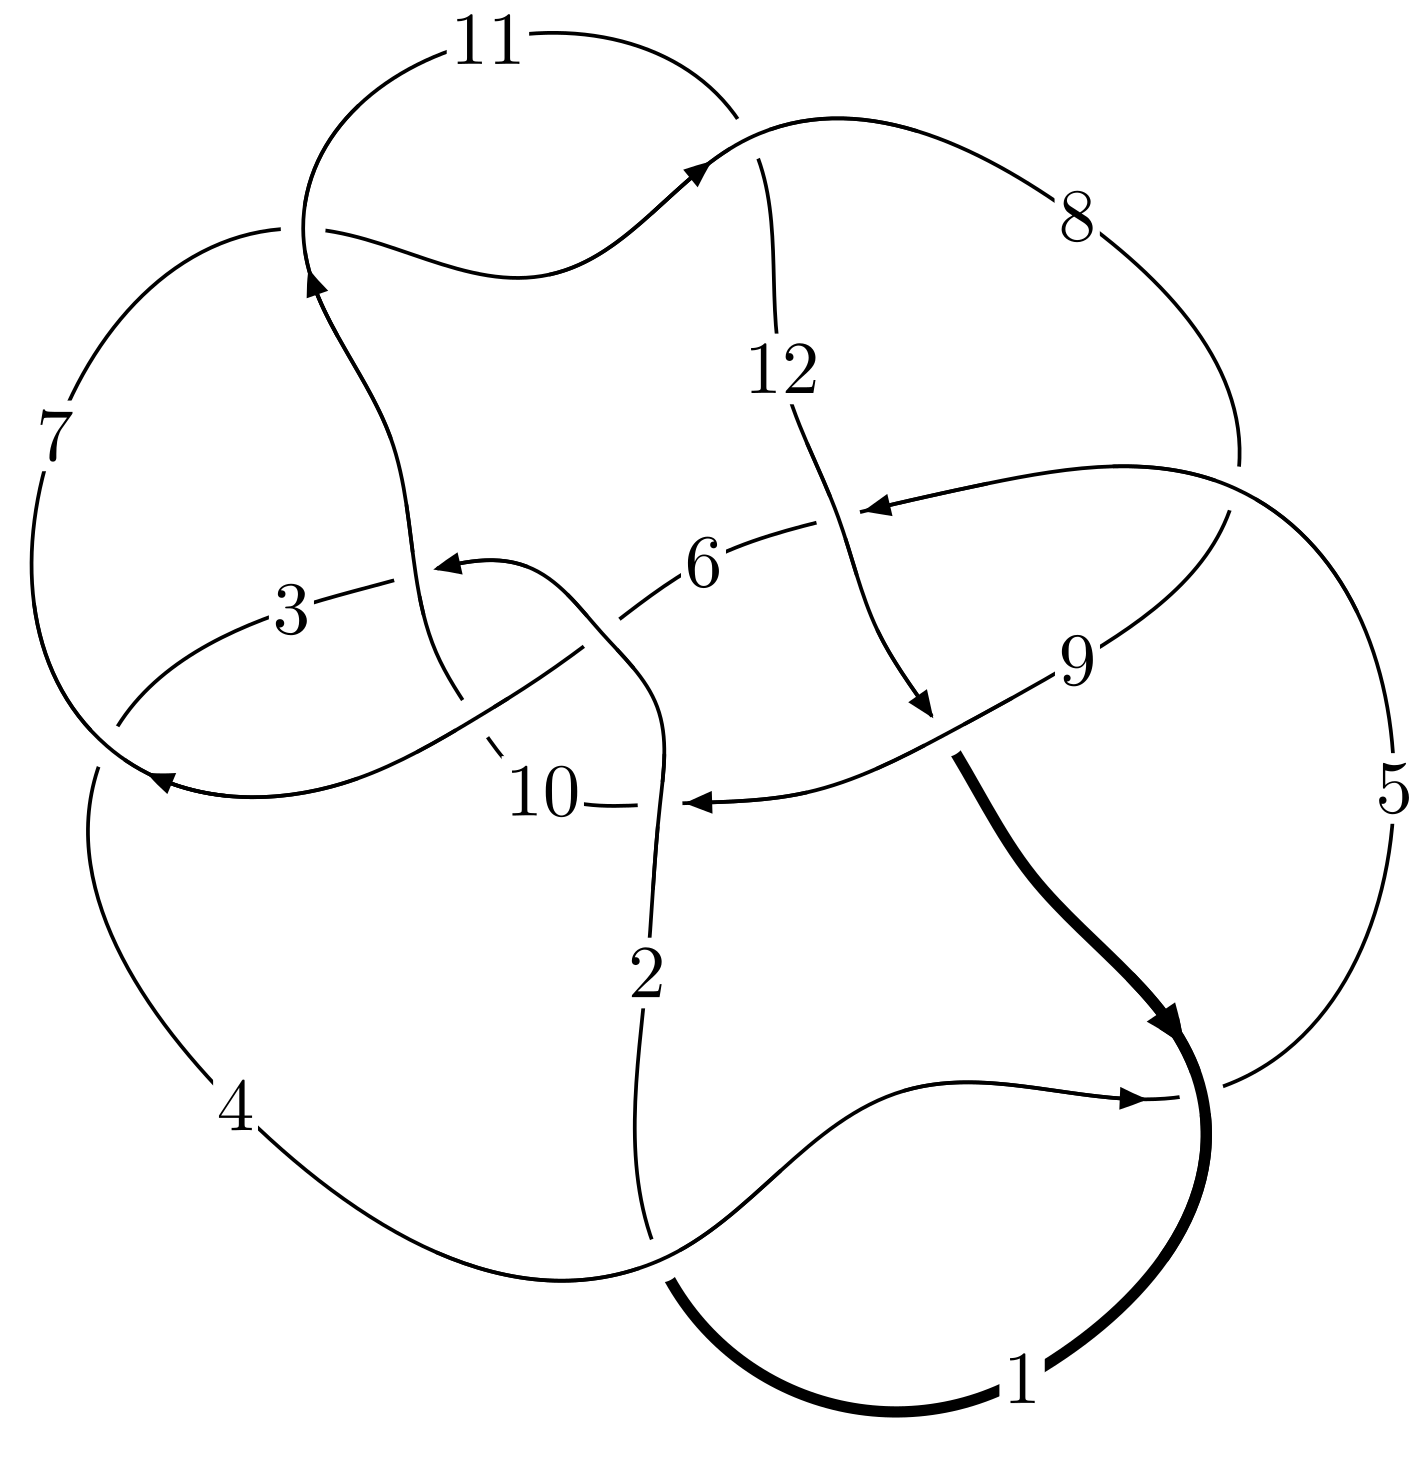
\includegraphics[width=112pt]{../../../GIT/diagram.site/Diagrams/png/2826_12n_0737.png}\\
\ \ \ A knot diagram\footnotemark}&
\allowdisplaybreaks
\textbf{Linearized knot diagam} \\
\cline{2-2}
 &
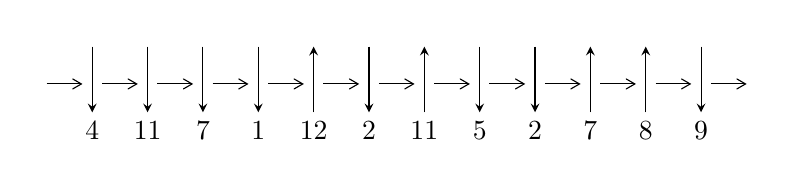
\begin{tikzpicture}[x=20pt, y=17pt]
	% nodes
	\node (C0) at (0, 0) {};
	\node (C1) at (1, 0) {};
	\node (C1U) at (1, +1) {};
	\node (C1D) at (1, -1) {4};

	\node (C2) at (2, 0) {};
	\node (C2U) at (2, +1) {};
	\node (C2D) at (2, -1) {11};

	\node (C3) at (3, 0) {};
	\node (C3U) at (3, +1) {};
	\node (C3D) at (3, -1) {7};

	\node (C4) at (4, 0) {};
	\node (C4U) at (4, +1) {};
	\node (C4D) at (4, -1) {1};

	\node (C5) at (5, 0) {};
	\node (C5U) at (5, +1) {};
	\node (C5D) at (5, -1) {12};

	\node (C6) at (6, 0) {};
	\node (C6U) at (6, +1) {};
	\node (C6D) at (6, -1) {2};

	\node (C7) at (7, 0) {};
	\node (C7U) at (7, +1) {};
	\node (C7D) at (7, -1) {11};

	\node (C8) at (8, 0) {};
	\node (C8U) at (8, +1) {};
	\node (C8D) at (8, -1) {5};

	\node (C9) at (9, 0) {};
	\node (C9U) at (9, +1) {};
	\node (C9D) at (9, -1) {2};

	\node (C10) at (10, 0) {};
	\node (C10U) at (10, +1) {};
	\node (C10D) at (10, -1) {7};

	\node (C11) at (11, 0) {};
	\node (C11U) at (11, +1) {};
	\node (C11D) at (11, -1) {8};

	\node (C12) at (12, 0) {};
	\node (C12U) at (12, +1) {};
	\node (C12D) at (12, -1) {9};
	\node (C13) at (13, 0) {};

	% arrows
	\draw[->,>={angle 60}]
	(C0) edge (C1) (C1) edge (C2) (C2) edge (C3) (C3) edge (C4) (C4) edge (C5) (C5) edge (C6) (C6) edge (C7) (C7) edge (C8) (C8) edge (C9) (C9) edge (C10) (C10) edge (C11) (C11) edge (C12) (C12) edge (C13) ;	\draw[->,>=stealth]
	(C1U) edge (C1D) (C2U) edge (C2D) (C3U) edge (C3D) (C4U) edge (C4D) (C5D) edge (C5U) (C6U) edge (C6D) (C7D) edge (C7U) (C8U) edge (C8D) (C9U) edge (C9D) (C10D) edge (C10U) (C11D) edge (C11U) (C12U) edge (C12D) ;
	\end{tikzpicture} \\
\hhline{~~} \\& 
\textbf{Solving Sequence} \\ \cline{2-2} 
 &
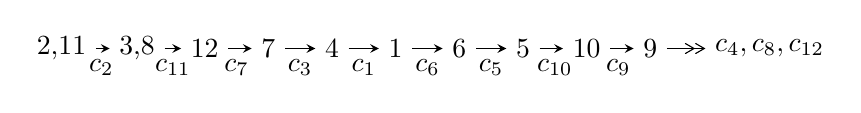
\begin{tikzpicture}[x=23pt, y=7pt]
	% node
	\node (A0) at (-1/8, 0) {2,11};
	\node (A1) at (17/16, 0) {3,8};
	\node (A2) at (17/8, 0) {12};
	\node (A3) at (25/8, 0) {7};
	\node (A4) at (33/8, 0) {4};
	\node (A5) at (41/8, 0) {1};
	\node (A6) at (49/8, 0) {6};
	\node (A7) at (57/8, 0) {5};
	\node (A8) at (65/8, 0) {10};
	\node (A9) at (73/8, 0) {9};
	\node (C1) at (1/2, -1) {$c_{2}$};
	\node (C2) at (13/8, -1) {$c_{11}$};
	\node (C3) at (21/8, -1) {$c_{7}$};
	\node (C4) at (29/8, -1) {$c_{3}$};
	\node (C5) at (37/8, -1) {$c_{1}$};
	\node (C6) at (45/8, -1) {$c_{6}$};
	\node (C7) at (53/8, -1) {$c_{5}$};
	\node (C8) at (61/8, -1) {$c_{10}$};
	\node (C9) at (69/8, -1) {$c_{9}$};
	\node (A10) at (11, 0) {$c_{4},c_{8},c_{12}$};

	% edge
	\draw[->,>=stealth]	
	(A0) edge (A1) (A1) edge (A2) (A2) edge (A3) (A3) edge (A4) (A4) edge (A5) (A5) edge (A6) (A6) edge (A7) (A7) edge (A8) (A8) edge (A9) ;
	\draw[->>,>={angle 60}]	
	(A9) edge (A10);
\end{tikzpicture} \\ 

\end{tabular} \\

\footnotetext{
The image of knot diagram is generated by the software ``\textbf{Draw programme}" developed by Andrew Bartholomew(\url{http://www.layer8.co.uk/maths/draw/index.htm\#Running-draw}), where we modified some parts for our purpose(\url{https://github.com/CATsTAILs/LinksPainter}).
}\phantom \\ \newline 
\centering \textbf{Ideals for irreducible components\footnotemark of $X_{\text{par}}$} 
 
\begin{align*}
I^u_{1}&=\langle 
b+u,\;-5.39993\times10^{21} u^{20}-1.73558\times10^{22} u^{19}+\cdots+2.47379\times10^{22} a-8.83120\times10^{22},\\
\phantom{I^u_{1}}&\phantom{= \langle  }u^{21}+25 u^{19}+\cdots+u+1\rangle \\
I^u_{2}&=\langle 
b+u,\;-3035105 u^{12}+837784 u^{11}+\cdots+1269257 a-4665416,\\
\phantom{I^u_{2}}&\phantom{= \langle  }u^{13}+4 u^{11}-3 u^{10}-14 u^9+14 u^8+30 u^7-27 u^6-9 u^5+24 u^4- u^3-6 u^2+2 u+1\rangle \\
I^u_{3}&=\langle 
-4.67268\times10^{23} u^{17}-1.17012\times10^{24} u^{16}+\cdots+4.11076\times10^{26} b-4.67615\times10^{26},\\
\phantom{I^u_{3}}&\phantom{= \langle  }9.23360\times10^{24} u^{17}+3.69267\times10^{25} u^{16}+\cdots+1.05852\times10^{28} a+1.11492\times10^{28},\\
\phantom{I^u_{3}}&\phantom{= \langle  }u^{18}+u^{17}+\cdots+512 u+206\rangle \\
I^u_{4}&=\langle 
b-1,\;2 a- u+2,\;u^2-2 u+2\rangle \\
I^u_{5}&=\langle 
b^2+2 b+2,\;a-1,\;u+1\rangle \\
\\
\end{align*}
\raggedright * 5 irreducible components of $\dim_{\mathbb{C}}=0$, with total 56 representations.\\
\footnotetext{All coefficients of polynomials are rational numbers. But the coefficients are sometimes approximated in decimal forms when there is not enough margin.}
\newpage
\renewcommand{\arraystretch}{1}
\centering \section*{I. $I^u_{1}= \langle b+u,\;-5.40\times10^{21} u^{20}-1.74\times10^{22} u^{19}+\cdots+2.47\times10^{22} a-8.83\times10^{22},\;u^{21}+25 u^{19}+\cdots+u+1 \rangle$}
\flushleft \textbf{(i) Arc colorings}\\
\begin{tabular}{m{7pt} m{180pt} m{7pt} m{180pt} }
\flushright $a_{2}=$&$\begin{pmatrix}1\\0\end{pmatrix}$ \\
\flushright $a_{11}=$&$\begin{pmatrix}0\\u\end{pmatrix}$ \\
\flushright $a_{3}=$&$\begin{pmatrix}1\\u^2\end{pmatrix}$ \\
\flushright $a_{8}=$&$\begin{pmatrix}0.218285 u^{20}+0.701585 u^{19}+\cdots+4.16608 u+3.56990\\- u\end{pmatrix}$ \\
\flushright $a_{12}=$&$\begin{pmatrix}-0.0236086 u^{20}-0.454671 u^{19}+\cdots-3.43605 u-1.12582\\-0.0461919 u^{20}+0.0773359 u^{19}+\cdots+1.91987 u+0.701585\end{pmatrix}$ \\
\flushright $a_{7}=$&$\begin{pmatrix}0.218285 u^{20}+0.701585 u^{19}+\cdots+4.16608 u+3.56990\\0.0461919 u^{20}-0.0773359 u^{19}+\cdots-1.91987 u-0.701585\end{pmatrix}$ \\
\flushright $a_{4}=$&$\begin{pmatrix}-0.701585 u^{20}-0.0461919 u^{19}+\cdots-3.35162 u+1.21829\\0.0773359 u^{20}-0.0368722 u^{19}+\cdots+0.747777 u+0.0461919\end{pmatrix}$ \\
\flushright $a_{1}=$&$\begin{pmatrix}-0.344227 u^{20}+0.127290 u^{19}+\cdots-2.85190 u+0.707526\\0.00198645 u^{20}-0.161647 u^{19}+\cdots+0.257401 u-0.164162\end{pmatrix}$ \\
\flushright $a_{6}=$&$\begin{pmatrix}0.264477 u^{20}+0.624249 u^{19}+\cdots+2.24621 u+2.86832\\0.0461919 u^{20}-0.0773359 u^{19}+\cdots-1.91987 u-0.701585\end{pmatrix}$ \\
\flushright $a_{5}=$&$\begin{pmatrix}-0.875790 u^{20}+0.451552 u^{19}+\cdots-5.00872 u+1.53539\\0.266657 u^{20}-0.0156100 u^{19}+\cdots+0.224114 u-0.576327\end{pmatrix}$ \\
\flushright $a_{10}=$&$\begin{pmatrix}0.0236086 u^{20}+0.454671 u^{19}+\cdots+3.43605 u+1.12582\\0.200090 u^{20}-0.189555 u^{19}+\cdots-0.398150 u-1.15626\end{pmatrix}$ \\
\flushright $a_{9}=$&$\begin{pmatrix}0.223699 u^{20}+0.265116 u^{19}+\cdots+3.03790 u-0.0304368\\0.200090 u^{20}-0.189555 u^{19}+\cdots-0.398150 u-1.15626\end{pmatrix}$\\&\end{tabular}
\flushleft \textbf{(ii) Obstruction class $= -1$}\\~\\
\flushleft \textbf{(iii) Cusp Shapes $= -\frac{34018566246715620144259}{12368961610252189857652} u^{20}-\frac{4694223251017745076299}{12368961610252189857652} u^{19}+\cdots-\frac{153162225510311692592391}{6184480805126094928826} u-\frac{44380162749147865603681}{12368961610252189857652}$}\\~\\
\newpage\renewcommand{\arraystretch}{1}
\flushleft \textbf{(iv) u-Polynomials at the component}\newline \\
\begin{tabular}{m{50pt}|m{274pt}}
Crossings & \hspace{64pt}u-Polynomials at each crossing \\
\hline $$\begin{aligned}c_{1},c_{4}\end{aligned}$$&$\begin{aligned}
&u^{21}-8 u^{20}+\cdots-22 u+2
\end{aligned}$\\
\hline $$\begin{aligned}c_{2},c_{3}\end{aligned}$$&$\begin{aligned}
&u^{21}+25 u^{19}+\cdots+u+1
\end{aligned}$\\
\hline $$\begin{aligned}c_{5}\end{aligned}$$&$\begin{aligned}
&u^{21}-19 u^{20}+\cdots-1856 u+256
\end{aligned}$\\
\hline $$\begin{aligned}c_{6}\end{aligned}$$&$\begin{aligned}
&u^{21}+u^{20}+\cdots+5 u+2
\end{aligned}$\\
\hline $$\begin{aligned}c_{7},c_{10},c_{11}\end{aligned}$$&$\begin{aligned}
&u^{21}-8 u^{20}+\cdots-26 u+10
\end{aligned}$\\
\hline $$\begin{aligned}c_{8},c_{12}\end{aligned}$$&$\begin{aligned}
&u^{21}+u^{20}+\cdots+6 u+1
\end{aligned}$\\
\hline $$\begin{aligned}c_{9}\end{aligned}$$&$\begin{aligned}
&u^{21}- u^{20}+\cdots+66 u+76
\end{aligned}$\\
\hline
\end{tabular}\\~\\
\newpage\renewcommand{\arraystretch}{1}
\flushleft \textbf{(v) Riley Polynomials at the component}\newline \\
\begin{tabular}{m{50pt}|m{274pt}}
Crossings & \hspace{64pt}Riley Polynomials at each crossing \\
\hline $$\begin{aligned}c_{1},c_{4}\end{aligned}$$&$\begin{aligned}
&y^{21}+16 y^{20}+\cdots+56 y-4
\end{aligned}$\\
\hline $$\begin{aligned}c_{2},c_{3}\end{aligned}$$&$\begin{aligned}
&y^{21}+50 y^{20}+\cdots-19 y-1
\end{aligned}$\\
\hline $$\begin{aligned}c_{5}\end{aligned}$$&$\begin{aligned}
&y^{21}-7 y^{20}+\cdots+348160 y-65536
\end{aligned}$\\
\hline $$\begin{aligned}c_{6}\end{aligned}$$&$\begin{aligned}
&y^{21}+43 y^{20}+\cdots-179 y-4
\end{aligned}$\\
\hline $$\begin{aligned}c_{7},c_{10},c_{11}\end{aligned}$$&$\begin{aligned}
&y^{21}-32 y^{20}+\cdots+1776 y-100
\end{aligned}$\\
\hline $$\begin{aligned}c_{8},c_{12}\end{aligned}$$&$\begin{aligned}
&y^{21}+11 y^{20}+\cdots+38 y-1
\end{aligned}$\\
\hline $$\begin{aligned}c_{9}\end{aligned}$$&$\begin{aligned}
&y^{21}+29 y^{20}+\cdots+6636 y-5776
\end{aligned}$\\
\hline
\end{tabular}\\~\\
\newpage\flushleft \textbf{(vi) Complex Volumes and Cusp Shapes}
$$\begin{array}{c|c|c}  
\text{Solutions to }I^u_{1}& \I (\text{vol} + \sqrt{-1}CS) & \text{Cusp shape}\\
 \hline 
\begin{aligned}
u &= \phantom{-}0.591384 + 0.684501 I \\
a &= \phantom{-}0.986086 - 0.952196 I \\
b &= -0.591384 - 0.684501 I\end{aligned}
 & \phantom{-}2.90718 + 0.62164 I & -0.21352 - 2.05306 I \\ \hline\begin{aligned}
u &= \phantom{-}0.591384 - 0.684501 I \\
a &= \phantom{-}0.986086 + 0.952196 I \\
b &= -0.591384 + 0.684501 I\end{aligned}
 & \phantom{-}2.90718 - 0.62164 I & -0.21352 + 2.05306 I \\ \hline\begin{aligned}
u &= \phantom{-}0.633459 + 0.554243 I \\
a &= \phantom{-}0.225131 - 0.559868 I \\
b &= -0.633459 - 0.554243 I\end{aligned}
 & \phantom{-}3.13654 - 0.77238 I & -1.08315 + 3.79652 I \\ \hline\begin{aligned}
u &= \phantom{-}0.633459 - 0.554243 I \\
a &= \phantom{-}0.225131 + 0.559868 I \\
b &= -0.633459 + 0.554243 I\end{aligned}
 & \phantom{-}3.13654 + 0.77238 I & -1.08315 - 3.79652 I \\ \hline\begin{aligned}
u &= -0.411221 + 0.734008 I \\
a &= -1.125200 - 0.068544 I \\
b &= \phantom{-}0.411221 - 0.734008 I\end{aligned}
 & \phantom{-}3.06565 - 2.80817 I & -0.13665 + 3.60000 I \\ \hline\begin{aligned}
u &= -0.411221 - 0.734008 I \\
a &= -1.125200 + 0.068544 I \\
b &= \phantom{-}0.411221 + 0.734008 I\end{aligned}
 & \phantom{-}3.06565 + 2.80817 I & -0.13665 - 3.60000 I \\ \hline\begin{aligned}
u &= \phantom{-}0.433795 + 0.519955 I \\
a &= -1.39067 + 1.14375 I \\
b &= -0.433795 - 0.519955 I\end{aligned}
 & \phantom{-}8.38211 - 0.33360 I & \phantom{-}5.43964 + 0.18682 I \\ \hline\begin{aligned}
u &= \phantom{-}0.433795 - 0.519955 I \\
a &= -1.39067 - 1.14375 I \\
b &= -0.433795 + 0.519955 I\end{aligned}
 & \phantom{-}8.38211 + 0.33360 I & \phantom{-}5.43964 - 0.18682 I \\ \hline\begin{aligned}
u &= -0.449539 + 0.447984 I \\
a &= \phantom{-}2.36305 + 0.92529 I \\
b &= \phantom{-}0.449539 - 0.447984 I\end{aligned}
 & \phantom{-}9.25551 - 8.18754 I & \phantom{-}2.61786 + 4.84295 I \\ \hline\begin{aligned}
u &= -0.449539 - 0.447984 I \\
a &= \phantom{-}2.36305 - 0.92529 I \\
b &= \phantom{-}0.449539 + 0.447984 I\end{aligned}
 & \phantom{-}9.25551 + 8.18754 I & \phantom{-}2.61786 - 4.84295 I\\
 \hline 
 \end{array}$$\newpage$$\begin{array}{c|c|c}  
\text{Solutions to }I^u_{1}& \I (\text{vol} + \sqrt{-1}CS) & \text{Cusp shape}\\
 \hline 
\begin{aligned}
u &= -0.610649\phantom{ +0.000000I} \\
a &= \phantom{-}0.463396\phantom{ +0.000000I} \\
b &= \phantom{-}0.610649\phantom{ +0.000000I}\end{aligned}
 & -1.19744\phantom{ +0.000000I} & -2.54880\phantom{ +0.000000I} \\ \hline\begin{aligned}
u &= \phantom{-}0.064145 + 0.480475 I \\
a &= -0.97482 + 2.36314 I \\
b &= -0.064145 - 0.480475 I\end{aligned}
 & \phantom{-}4.25500 + 4.70062 I & \phantom{-}0.78101 - 5.95257 I \\ \hline\begin{aligned}
u &= \phantom{-}0.064145 - 0.480475 I \\
a &= -0.97482 - 2.36314 I \\
b &= -0.064145 + 0.480475 I\end{aligned}
 & \phantom{-}4.25500 - 4.70062 I & \phantom{-}0.78101 + 5.95257 I \\ \hline\begin{aligned}
u &= -0.118660 + 0.375406 I \\
a &= \phantom{-}1.27547 - 0.90971 I \\
b &= \phantom{-}0.118660 - 0.375406 I\end{aligned}
 & -0.104584 + 1.401550 I & -1.22515 - 5.35896 I \\ \hline\begin{aligned}
u &= -0.118660 - 0.375406 I \\
a &= \phantom{-}1.27547 + 0.90971 I \\
b &= \phantom{-}0.118660 + 0.375406 I\end{aligned}
 & -0.104584 - 1.401550 I & -1.22515 + 5.35896 I \\ \hline\begin{aligned}
u &= -0.02275 + 2.82542 I \\
a &= \phantom{-}0.063198 - 0.686482 I \\
b &= \phantom{-}0.02275 - 2.82542 I\end{aligned}
 & -17.8874 + 12.7180 I & \phantom{-0.000000 } 0 \\ \hline\begin{aligned}
u &= -0.02275 - 2.82542 I \\
a &= \phantom{-}0.063198 + 0.686482 I \\
b &= \phantom{-}0.02275 + 2.82542 I\end{aligned}
 & -17.8874 - 12.7180 I & \phantom{-0.000000 } 0 \\ \hline\begin{aligned}
u &= -0.62719 + 2.81445 I \\
a &= -0.180831 - 0.609250 I \\
b &= \phantom{-}0.62719 - 2.81445 I\end{aligned}
 & \phantom{-}19.4705 - 1.7019 I & \phantom{-0.000000 } 0 \\ \hline\begin{aligned}
u &= -0.62719 - 2.81445 I \\
a &= -0.180831 + 0.609250 I \\
b &= \phantom{-}0.62719 + 2.81445 I\end{aligned}
 & \phantom{-}19.4705 + 1.7019 I & \phantom{-0.000000 } 0 \\ \hline\begin{aligned}
u &= \phantom{-}0.21191 + 2.98201 I \\
a &= \phantom{-}0.026904 - 0.620788 I \\
b &= -0.21191 - 2.98201 I\end{aligned}
 & \phantom{-}15.8213 - 6.2554 I & \phantom{-0.000000 } 0\\
 \hline 
 \end{array}$$\newpage$$\begin{array}{c|c|c}  
\text{Solutions to }I^u_{1}& \I (\text{vol} + \sqrt{-1}CS) & \text{Cusp shape}\\
 \hline 
\begin{aligned}
u &= \phantom{-}0.21191 - 2.98201 I \\
a &= \phantom{-}0.026904 + 0.620788 I \\
b &= -0.21191 + 2.98201 I\end{aligned}
 & \phantom{-}15.8213 + 6.2554 I & \phantom{-0.000000 } 0\\
 \hline 
 \end{array}$$\newpage\newpage\renewcommand{\arraystretch}{1}
\centering \section*{II. $I^u_{2}= \langle b+u,\;-3.04\times10^{6} u^{12}+8.38\times10^{5} u^{11}+\cdots+1.27\times10^{6} a-4.67\times10^{6},\;u^{13}+4 u^{11}+\cdots+2 u+1 \rangle$}
\flushleft \textbf{(i) Arc colorings}\\
\begin{tabular}{m{7pt} m{180pt} m{7pt} m{180pt} }
\flushright $a_{2}=$&$\begin{pmatrix}1\\0\end{pmatrix}$ \\
\flushright $a_{11}=$&$\begin{pmatrix}0\\u\end{pmatrix}$ \\
\flushright $a_{3}=$&$\begin{pmatrix}1\\u^2\end{pmatrix}$ \\
\flushright $a_{8}=$&$\begin{pmatrix}2.39125 u^{12}-0.660059 u^{11}+\cdots-9.61560 u+3.67571\\- u\end{pmatrix}$ \\
\flushright $a_{12}=$&$\begin{pmatrix}-2.96162 u^{12}+1.00248 u^{11}+\cdots+12.9399 u-5.17648\\-0.0312159 u^{12}+0.392917 u^{11}+\cdots+2.07113 u-0.660059\end{pmatrix}$ \\
\flushright $a_{7}=$&$\begin{pmatrix}2.39125 u^{12}-0.660059 u^{11}+\cdots-9.61560 u+3.67571\\0.0312159 u^{12}-0.392917 u^{11}+\cdots-2.07113 u+0.660059\end{pmatrix}$ \\
\flushright $a_{4}=$&$\begin{pmatrix}0.660059 u^{12}-0.0312159 u^{11}+\cdots+1.10678 u+3.39125\\0.392917 u^{12}+0.0508833 u^{11}+\cdots-0.597627 u+0.0312159\end{pmatrix}$ \\
\flushright $a_{1}=$&$\begin{pmatrix}-1.65839 u^{12}-0.257842 u^{11}+\cdots+2.91119 u+0.964264\\-0.424133 u^{12}+0.342034 u^{11}+\cdots+2.66876 u+0.308725\end{pmatrix}$ \\
\flushright $a_{6}=$&$\begin{pmatrix}2.42246 u^{12}-1.05298 u^{11}+\cdots-11.6867 u+4.33576\\0.0312159 u^{12}-0.392917 u^{11}+\cdots-2.07113 u+0.660059\end{pmatrix}$ \\
\flushright $a_{5}=$&$\begin{pmatrix}1.26999 u^{12}-1.05851 u^{11}+\cdots-6.41247 u+2.32712\\0.166291 u^{12}-0.668395 u^{11}+\cdots+0.612283 u+1.34966\end{pmatrix}$ \\
\flushright $a_{10}=$&$\begin{pmatrix}2.96162 u^{12}-1.00248 u^{11}+\cdots-12.9399 u+5.17648\\-0.0266959 u^{12}-0.872552 u^{11}+\cdots-1.02779 u+1.66254\end{pmatrix}$ \\
\flushright $a_{9}=$&$\begin{pmatrix}2.93493 u^{12}-1.87504 u^{11}+\cdots-13.9677 u+6.83902\\-0.0266959 u^{12}-0.872552 u^{11}+\cdots-1.02779 u+1.66254\end{pmatrix}$\\&\end{tabular}
\flushleft \textbf{(ii) Obstruction class $= 1$}\\~\\
\flushleft \textbf{(iii) Cusp Shapes $= -\frac{11098661}{1269257} u^{12}+\frac{5890928}{1269257} u^{11}+\cdots+\frac{9880480}{1269257} u-\frac{16615848}{1269257}$}\\~\\
\newpage\renewcommand{\arraystretch}{1}
\flushleft \textbf{(iv) u-Polynomials at the component}\newline \\
\begin{tabular}{m{50pt}|m{274pt}}
Crossings & \hspace{64pt}u-Polynomials at each crossing \\
\hline $$\begin{aligned}c_{1}\end{aligned}$$&$\begin{aligned}
&u^{13}-5 u^{12}+\cdots+27 u-4
\end{aligned}$\\
\hline $$\begin{aligned}c_{2}\end{aligned}$$&$\begin{aligned}
&u^{13}+4 u^{11}+\cdots+2 u+1
\end{aligned}$\\
\hline $$\begin{aligned}c_{3}\end{aligned}$$&$\begin{aligned}
&u^{13}+4 u^{11}+\cdots+2 u-1
\end{aligned}$\\
\hline $$\begin{aligned}c_{4}\end{aligned}$$&$\begin{aligned}
&u^{13}+5 u^{12}+\cdots+27 u+4
\end{aligned}$\\
\hline $$\begin{aligned}c_{5}\end{aligned}$$&$\begin{aligned}
&u^{13}+6 u^{12}+\cdots+u-1
\end{aligned}$\\
\hline $$\begin{aligned}c_{6}\end{aligned}$$&$\begin{aligned}
&u^{13}- u^{12}+\cdots- u+1
\end{aligned}$\\
\hline $$\begin{aligned}c_{7}\end{aligned}$$&$\begin{aligned}
&u^{13}-5 u^{12}+\cdots+3 u+2
\end{aligned}$\\
\hline $$\begin{aligned}c_{8},c_{12}\end{aligned}$$&$\begin{aligned}
&u^{13}- u^{12}+u^{11}+u^{10}+2 u^9-3 u^8+u^7+3 u^6- u^5-2 u^4+2 u^3- u-1
\end{aligned}$\\
\hline $$\begin{aligned}c_{9}\end{aligned}$$&$\begin{aligned}
&u^{13}- u^{12}+6 u^{11}+u^{10}+12 u^9+10 u^8+9 u^7+7 u^6+6 u^4+3 u^3-3 u^2+1
\end{aligned}$\\
\hline $$\begin{aligned}c_{10},c_{11}\end{aligned}$$&$\begin{aligned}
&u^{13}+5 u^{12}+\cdots+3 u-2
\end{aligned}$\\
\hline
\end{tabular}\\~\\
\newpage\renewcommand{\arraystretch}{1}
\flushleft \textbf{(v) Riley Polynomials at the component}\newline \\
\begin{tabular}{m{50pt}|m{274pt}}
Crossings & \hspace{64pt}Riley Polynomials at each crossing \\
\hline $$\begin{aligned}c_{1},c_{4}\end{aligned}$$&$\begin{aligned}
&y^{13}+9 y^{12}+\cdots+97 y-16
\end{aligned}$\\
\hline $$\begin{aligned}c_{2},c_{3}\end{aligned}$$&$\begin{aligned}
&y^{13}+8 y^{12}+\cdots+16 y-1
\end{aligned}$\\
\hline $$\begin{aligned}c_{5}\end{aligned}$$&$\begin{aligned}
&y^{13}-6 y^{12}+\cdots+7 y-1
\end{aligned}$\\
\hline $$\begin{aligned}c_{6}\end{aligned}$$&$\begin{aligned}
&y^{13}+9 y^{12}+\cdots+11 y-1
\end{aligned}$\\
\hline $$\begin{aligned}c_{7},c_{10},c_{11}\end{aligned}$$&$\begin{aligned}
&y^{13}-19 y^{12}+\cdots-11 y-4
\end{aligned}$\\
\hline $$\begin{aligned}c_{8},c_{12}\end{aligned}$$&$\begin{aligned}
&y^{13}+y^{12}+\cdots+y-1
\end{aligned}$\\
\hline $$\begin{aligned}c_{9}\end{aligned}$$&$\begin{aligned}
&y^{13}+11 y^{12}+\cdots+6 y-1
\end{aligned}$\\
\hline
\end{tabular}\\~\\
\newpage\flushleft \textbf{(vi) Complex Volumes and Cusp Shapes}
$$\begin{array}{c|c|c}  
\text{Solutions to }I^u_{2}& \I (\text{vol} + \sqrt{-1}CS) & \text{Cusp shape}\\
 \hline 
\begin{aligned}
u &= \phantom{-}0.584682 + 0.557508 I \\
a &= \phantom{-}0.467799 + 0.459309 I \\
b &= -0.584682 - 0.557508 I\end{aligned}
 & \phantom{-}1.87818 - 5.16888 I & -5.45109 + 5.60438 I \\ \hline\begin{aligned}
u &= \phantom{-}0.584682 - 0.557508 I \\
a &= \phantom{-}0.467799 - 0.459309 I \\
b &= -0.584682 + 0.557508 I\end{aligned}
 & \phantom{-}1.87818 + 5.16888 I & -5.45109 - 5.60438 I \\ \hline\begin{aligned}
u &= -0.646836 + 0.067688 I \\
a &= \phantom{-}0.529126 - 0.404517 I \\
b &= \phantom{-}0.646836 - 0.067688 I\end{aligned}
 & -1.42512 - 0.47239 I & -7.52545 + 9.55816 I \\ \hline\begin{aligned}
u &= -0.646836 - 0.067688 I \\
a &= \phantom{-}0.529126 + 0.404517 I \\
b &= \phantom{-}0.646836 + 0.067688 I\end{aligned}
 & -1.42512 + 0.47239 I & -7.52545 - 9.55816 I \\ \hline\begin{aligned}
u &= \phantom{-}0.498804 + 0.404257 I \\
a &= -2.04698 + 0.60897 I \\
b &= -0.498804 - 0.404257 I\end{aligned}
 & \phantom{-}6.09438 - 1.34909 I & \phantom{-}0.36538 + 1.86326 I \\ \hline\begin{aligned}
u &= \phantom{-}0.498804 - 0.404257 I \\
a &= -2.04698 - 0.60897 I \\
b &= -0.498804 + 0.404257 I\end{aligned}
 & \phantom{-}6.09438 + 1.34909 I & \phantom{-}0.36538 - 1.86326 I \\ \hline\begin{aligned}
u &= -1.254250 + 0.588394 I \\
a &= -0.840675 - 0.538825 I \\
b &= \phantom{-}1.254250 - 0.588394 I\end{aligned}
 & \phantom{-}6.40935 + 7.59409 I & \phantom{-}1.22194 - 5.34686 I \\ \hline\begin{aligned}
u &= -1.254250 - 0.588394 I \\
a &= -0.840675 + 0.538825 I \\
b &= \phantom{-}1.254250 + 0.588394 I\end{aligned}
 & \phantom{-}6.40935 - 7.59409 I & \phantom{-}1.22194 + 5.34686 I \\ \hline\begin{aligned}
u &= \phantom{-}1.245380 + 0.642473 I \\
a &= \phantom{-}0.984992 - 0.368357 I \\
b &= -1.245380 - 0.642473 I\end{aligned}
 & \phantom{-}4.54418 + 2.44460 I & \phantom{-}2.99018 - 2.95945 I \\ \hline\begin{aligned}
u &= \phantom{-}1.245380 - 0.642473 I \\
a &= \phantom{-}0.984992 + 0.368357 I \\
b &= -1.245380 + 0.642473 I\end{aligned}
 & \phantom{-}4.54418 - 2.44460 I & \phantom{-}2.99018 + 2.95945 I\\
 \hline 
 \end{array}$$\newpage$$\begin{array}{c|c|c}  
\text{Solutions to }I^u_{2}& \I (\text{vol} + \sqrt{-1}CS) & \text{Cusp shape}\\
 \hline 
\begin{aligned}
u &= -0.328910\phantom{ +0.000000I} \\
a &= \phantom{-}4.07049\phantom{ +0.000000I} \\
b &= \phantom{-}0.328910\phantom{ +0.000000I}\end{aligned}
 & \phantom{-}1.84881\phantom{ +0.000000I} & -6.67710\phantom{ +0.000000I} \\ \hline\begin{aligned}
u &= -0.26332 + 2.64930 I \\
a &= -0.129510 - 0.704018 I \\
b &= \phantom{-}0.26332 - 2.64930 I\end{aligned}
 & \phantom{-}17.7632 - 2.2039 I & \phantom{-}0.237574 + 0.419872 I \\ \hline\begin{aligned}
u &= -0.26332 - 2.64930 I \\
a &= -0.129510 + 0.704018 I \\
b &= \phantom{-}0.26332 + 2.64930 I\end{aligned}
 & \phantom{-}17.7632 + 2.2039 I & \phantom{-}0.237574 - 0.419872 I\\
 \hline 
 \end{array}$$\newpage\newpage\renewcommand{\arraystretch}{1}
\centering \section*{III. $I^u_{3}= \langle -4.67\times10^{23} u^{17}-1.17\times10^{24} u^{16}+\cdots+4.11\times10^{26} b-4.68\times10^{26},\;9.23\times10^{24} u^{17}+3.69\times10^{25} u^{16}+\cdots+1.06\times10^{28} a+1.11\times10^{28},\;u^{18}+u^{17}+\cdots+512 u+206 \rangle$}
\flushleft \textbf{(i) Arc colorings}\\
\begin{tabular}{m{7pt} m{180pt} m{7pt} m{180pt} }
\flushright $a_{2}=$&$\begin{pmatrix}1\\0\end{pmatrix}$ \\
\flushright $a_{11}=$&$\begin{pmatrix}0\\u\end{pmatrix}$ \\
\flushright $a_{3}=$&$\begin{pmatrix}1\\u^2\end{pmatrix}$ \\
\flushright $a_{8}=$&$\begin{pmatrix}-0.000872310 u^{17}-0.00348851 u^{16}+\cdots-0.911938 u-1.05328\\0.00113669 u^{17}+0.00284649 u^{16}+\cdots+0.0571899 u+1.13754\end{pmatrix}$ \\
\flushright $a_{12}=$&$\begin{pmatrix}-0.00619818 u^{17}-0.00659840 u^{16}+\cdots-3.79065 u-2.55336\\-0.000735882 u^{17}+0.00238650 u^{16}+\cdots+0.849826 u+0.901098\end{pmatrix}$ \\
\flushright $a_{7}=$&$\begin{pmatrix}-0.000872310 u^{17}-0.00348851 u^{16}+\cdots-0.911938 u-1.05328\\0.00337890 u^{17}+0.00352881 u^{16}+\cdots+1.57638 u+1.67648\end{pmatrix}$ \\
\flushright $a_{4}=$&$\begin{pmatrix}-0.00437426 u^{17}-0.00511014 u^{16}+\cdots-3.81879 u-1.38980\\0.00392577 u^{17}+0.00295684 u^{16}+\cdots+1.78231 u+1.86297\end{pmatrix}$ \\
\flushright $a_{1}=$&$\begin{pmatrix}0.00326686 u^{17}-0.00265625 u^{16}+\cdots+2.02077 u-1.22406\\-0.00672287 u^{17}-0.00269067 u^{16}+\cdots-2.56234 u-1.01072\end{pmatrix}$ \\
\flushright $a_{6}=$&$\begin{pmatrix}0.00250659 u^{17}+0.0000402959 u^{16}+\cdots+0.664442 u+0.623194\\0.00337890 u^{17}+0.00352881 u^{16}+\cdots+1.57638 u+1.67648\end{pmatrix}$ \\
\flushright $a_{5}=$&$\begin{pmatrix}0.00870477 u^{17}+0.00663870 u^{16}+\cdots+4.45509 u+3.17656\\0.00411478 u^{17}+0.00114230 u^{16}+\cdots+0.726555 u+0.775377\end{pmatrix}$ \\
\flushright $a_{10}=$&$\begin{pmatrix}0.00619818 u^{17}+0.00659840 u^{16}+\cdots+3.79065 u+2.55336\\-0.00116233 u^{17}-0.00210654 u^{16}+\cdots-0.331565 u-0.983544\end{pmatrix}$ \\
\flushright $a_{9}=$&$\begin{pmatrix}0.00503585 u^{17}+0.00449186 u^{16}+\cdots+3.45908 u+1.56982\\-0.00116233 u^{17}-0.00210654 u^{16}+\cdots-0.331565 u-0.983544\end{pmatrix}$\\&\end{tabular}
\flushleft \textbf{(ii) Obstruction class $= -1$}\\~\\
\flushleft \textbf{(iii) Cusp Shapes $= -\frac{2356314796722538609456367}{205538248502201329427999196} u^{17}-\frac{197356226700656101872041}{102769124251100664713999598} u^{16}+\cdots-\frac{644603608722482183906910875}{102769124251100664713999598} u+\frac{7790438242139030196174041}{102769124251100664713999598}$}\\~\\
\newpage\renewcommand{\arraystretch}{1}
\flushleft \textbf{(iv) u-Polynomials at the component}\newline \\
\begin{tabular}{m{50pt}|m{274pt}}
Crossings & \hspace{64pt}u-Polynomials at each crossing \\
\hline $$\begin{aligned}c_{1},c_{4}\end{aligned}$$&$\begin{aligned}
&(u^9+u^8+5 u^7+4 u^6+8 u^5+5 u^4+2 u^3+u^2-4 u-1)^2
\end{aligned}$\\
\hline $$\begin{aligned}c_{2},c_{3}\end{aligned}$$&$\begin{aligned}
&u^{18}+u^{17}+\cdots+512 u+206
\end{aligned}$\\
\hline $$\begin{aligned}c_{5}\end{aligned}$$&$\begin{aligned}
&(u+1)^{18}
\end{aligned}$\\
\hline $$\begin{aligned}c_{6}\end{aligned}$$&$\begin{aligned}
&u^{18}- u^{17}+\cdots-532 u+401
\end{aligned}$\\
\hline $$\begin{aligned}c_{7},c_{10},c_{11}\end{aligned}$$&$\begin{aligned}
&(u^9+3 u^8-3 u^7-12 u^6+6 u^5+21 u^4-2 u^3-11 u^2-6 u-1)^2
\end{aligned}$\\
\hline $$\begin{aligned}c_{8},c_{12}\end{aligned}$$&$\begin{aligned}
&u^{18}+3 u^{17}+\cdots+8 u+2
\end{aligned}$\\
\hline $$\begin{aligned}c_{9}\end{aligned}$$&$\begin{aligned}
&u^{18}- u^{17}+\cdots+3168 u+1504
\end{aligned}$\\
\hline
\end{tabular}\\~\\
\newpage\renewcommand{\arraystretch}{1}
\flushleft \textbf{(v) Riley Polynomials at the component}\newline \\
\begin{tabular}{m{50pt}|m{274pt}}
Crossings & \hspace{64pt}Riley Polynomials at each crossing \\
\hline $$\begin{aligned}c_{1},c_{4}\end{aligned}$$&$\begin{aligned}
&(y^9+9 y^8+33 y^7+58 y^6+34 y^5-39 y^4-62 y^3-7 y^2+18 y-1)^2
\end{aligned}$\\
\hline $$\begin{aligned}c_{2},c_{3}\end{aligned}$$&$\begin{aligned}
&y^{18}+37 y^{17}+\cdots-103112 y+42436
\end{aligned}$\\
\hline $$\begin{aligned}c_{5}\end{aligned}$$&$\begin{aligned}
&(y-1)^{18}
\end{aligned}$\\
\hline $$\begin{aligned}c_{6}\end{aligned}$$&$\begin{aligned}
&y^{18}+39 y^{17}+\cdots+109154 y+160801
\end{aligned}$\\
\hline $$\begin{aligned}c_{7},c_{10},c_{11}\end{aligned}$$&$\begin{aligned}
&(y^9-15 y^8+\cdots+14 y-1)^{2}
\end{aligned}$\\
\hline $$\begin{aligned}c_{8},c_{12}\end{aligned}$$&$\begin{aligned}
&y^{18}+y^{17}+\cdots+72 y+4
\end{aligned}$\\
\hline $$\begin{aligned}c_{9}\end{aligned}$$&$\begin{aligned}
&y^{18}+25 y^{17}+\cdots-7100416 y+2262016
\end{aligned}$\\
\hline
\end{tabular}\\~\\
\newpage\flushleft \textbf{(vi) Complex Volumes and Cusp Shapes}
$$\begin{array}{c|c|c}  
\text{Solutions to }I^u_{3}& \I (\text{vol} + \sqrt{-1}CS) & \text{Cusp shape}\\
 \hline 
\begin{aligned}
u &= \phantom{-}0.886434 + 0.371388 I \\
a &= \phantom{-}1.096950 - 0.459588 I \\
b &= -0.886434 + 0.371388 I\end{aligned}
 & \phantom{-}3.15999\phantom{ +0.000000I} & -1.78243 + 0. I\phantom{ +0.000000I} \\ \hline\begin{aligned}
u &= \phantom{-}0.886434 - 0.371388 I \\
a &= \phantom{-}1.096950 + 0.459588 I \\
b &= -0.886434 - 0.371388 I\end{aligned}
 & \phantom{-}3.15999\phantom{ +0.000000I} & -1.78243 + 0. I\phantom{ +0.000000I} \\ \hline\begin{aligned}
u &= \phantom{-}0.205642 + 0.879714 I \\
a &= \phantom{-}0.257101 + 0.425056 I \\
b &= -1.095690 + 0.759227 I\end{aligned}
 & \phantom{-}2.95021 + 4.83805 I & \phantom{-}3.38372 - 2.81539 I \\ \hline\begin{aligned}
u &= \phantom{-}0.205642 - 0.879714 I \\
a &= \phantom{-}0.257101 - 0.425056 I \\
b &= -1.095690 - 0.759227 I\end{aligned}
 & \phantom{-}2.95021 - 4.83805 I & \phantom{-}3.38372 + 2.81539 I \\ \hline\begin{aligned}
u &= -0.653145 + 0.189006 I \\
a &= \phantom{-}0.414794 + 0.120032 I \\
b &= \phantom{-}0.653145 + 0.189006 I\end{aligned}
 & -1.18935\phantom{ +0.000000I} &                  -6
-0.171800 + 0. 10   I\phantom{ +0.000000I} \\ \hline\begin{aligned}
u &= -0.653145 - 0.189006 I \\
a &= \phantom{-}0.414794 - 0.120032 I \\
b &= \phantom{-}0.653145 - 0.189006 I\end{aligned}
 & -1.18935\phantom{ +0.000000I} &                  -6
-0.171800 + 0. 10   I\phantom{ +0.000000I} \\ \hline\begin{aligned}
u &= \phantom{-}1.095690 + 0.759227 I \\
a &= -0.331949 - 0.056184 I \\
b &= -0.205642 + 0.879714 I\end{aligned}
 & \phantom{-}2.95021 - 4.83805 I & \phantom{-}3.38372 + 2.81539 I \\ \hline\begin{aligned}
u &= \phantom{-}1.095690 - 0.759227 I \\
a &= -0.331949 + 0.056184 I \\
b &= -0.205642 - 0.879714 I\end{aligned}
 & \phantom{-}2.95021 + 4.83805 I & \phantom{-}3.38372 - 2.81539 I \\ \hline\begin{aligned}
u &= -0.419711 + 0.477941 I \\
a &= -0.60540 - 2.16213 I \\
b &= \phantom{-}1.40135 + 0.64766 I\end{aligned}
 & \phantom{-}7.78134 - 1.20594 I & \phantom{-}6.24179 + 1.20422 I \\ \hline\begin{aligned}
u &= -0.419711 - 0.477941 I \\
a &= -0.60540 + 2.16213 I \\
b &= \phantom{-}1.40135 - 0.64766 I\end{aligned}
 & \phantom{-}7.78134 + 1.20594 I & \phantom{-}6.24179 - 1.20422 I\\
 \hline 
 \end{array}$$\newpage$$\begin{array}{c|c|c}  
\text{Solutions to }I^u_{3}& \I (\text{vol} + \sqrt{-1}CS) & \text{Cusp shape}\\
 \hline 
\begin{aligned}
u &= -1.40135 + 0.64766 I \\
a &= -0.925008 + 0.013582 I \\
b &= \phantom{-}0.419711 + 0.477941 I\end{aligned}
 & \phantom{-}7.78134 + 1.20594 I & \phantom{-}6.24179 - 1.20422 I \\ \hline\begin{aligned}
u &= -1.40135 - 0.64766 I \\
a &= -0.925008 - 0.013582 I \\
b &= \phantom{-}0.419711 - 0.477941 I\end{aligned}
 & \phantom{-}7.78134 - 1.20594 I & \phantom{-}6.24179 + 1.20422 I \\ \hline\begin{aligned}
u &= -0.22580 + 2.48577 I \\
a &= \phantom{-}0.159711 + 0.767946 I \\
b &= \phantom{-}0.15187 + 2.78180 I\end{aligned}
 & \phantom{-}19.3983 - 3.3753 I & \phantom{-}4.74375 + 2.72891 I \\ \hline\begin{aligned}
u &= -0.22580 - 2.48577 I \\
a &= \phantom{-}0.159711 - 0.767946 I \\
b &= \phantom{-}0.15187 - 2.78180 I\end{aligned}
 & \phantom{-}19.3983 + 3.3753 I & \phantom{-}4.74375 - 2.72891 I \\ \hline\begin{aligned}
u &= \phantom{-}0.16411 + 2.66586 I \\
a &= -0.043531 + 0.707136 I \\
b &= -0.16411 + 2.66586 I\end{aligned}
 & \phantom{-}15.0815\phantom{ +0.000000I} &                  -6
-0.784284 + 0. 10   I\phantom{ +0.000000I} \\ \hline\begin{aligned}
u &= \phantom{-}0.16411 - 2.66586 I \\
a &= -0.043531 - 0.707136 I \\
b &= -0.16411 - 2.66586 I\end{aligned}
 & \phantom{-}15.0815\phantom{ +0.000000I} &                  -6
-0.784284 + 0. 10   I\phantom{ +0.000000I} \\ \hline\begin{aligned}
u &= -0.15187 + 2.78180 I \\
a &= -0.042083 + 0.701486 I \\
b &= \phantom{-}0.22580 + 2.48577 I\end{aligned}
 & \phantom{-}19.3983 + 3.3753 I & \phantom{-}4.74375 - 2.72891 I \\ \hline\begin{aligned}
u &= -0.15187 - 2.78180 I \\
a &= -0.042083 - 0.701486 I \\
b &= \phantom{-}0.22580 - 2.48577 I\end{aligned}
 & \phantom{-}19.3983 - 3.3753 I & \phantom{-}4.74375 + 2.72891 I\\
 \hline 
 \end{array}$$\newpage\newpage\renewcommand{\arraystretch}{1}
\centering \section*{IV. $I^u_{4}= \langle b-1,\;2 a- u+2,\;u^2-2 u+2 \rangle$}
\flushleft \textbf{(i) Arc colorings}\\
\begin{tabular}{m{7pt} m{180pt} m{7pt} m{180pt} }
\flushright $a_{2}=$&$\begin{pmatrix}1\\0\end{pmatrix}$ \\
\flushright $a_{11}=$&$\begin{pmatrix}0\\u\end{pmatrix}$ \\
\flushright $a_{3}=$&$\begin{pmatrix}1\\2 u-2\end{pmatrix}$ \\
\flushright $a_{8}=$&$\begin{pmatrix}\frac{1}{2} u-1\\1\end{pmatrix}$ \\
\flushright $a_{12}=$&$\begin{pmatrix}-\frac{1}{2} u+1\\u-1\end{pmatrix}$ \\
\flushright $a_{7}=$&$\begin{pmatrix}\frac{1}{2} u-1\\- u+1\end{pmatrix}$ \\
\flushright $a_{4}=$&$\begin{pmatrix}\frac{1}{2} u\\u-1\end{pmatrix}$ \\
\flushright $a_{1}=$&$\begin{pmatrix}-\frac{1}{2} u+2\\1\end{pmatrix}$ \\
\flushright $a_{6}=$&$\begin{pmatrix}-\frac{1}{2} u\\- u+1\end{pmatrix}$ \\
\flushright $a_{5}=$&$\begin{pmatrix}- u+1\\0\end{pmatrix}$ \\
\flushright $a_{10}=$&$\begin{pmatrix}\frac{1}{2} u-1\\1\end{pmatrix}$ \\
\flushright $a_{9}=$&$\begin{pmatrix}\frac{1}{2} u\\1\end{pmatrix}$\\&\end{tabular}
\flushleft \textbf{(ii) Obstruction class $= 1$}\\~\\
\flushleft \textbf{(iii) Cusp Shapes $= 4$}\\~\\
\newpage\renewcommand{\arraystretch}{1}
\flushleft \textbf{(iv) u-Polynomials at the component}\newline \\
\begin{tabular}{m{50pt}|m{274pt}}
Crossings & \hspace{64pt}u-Polynomials at each crossing \\
\hline $$\begin{aligned}c_{1},c_{4},c_{6}\\c_{8}\end{aligned}$$&$\begin{aligned}
&u^2+1
\end{aligned}$\\
\hline $$\begin{aligned}c_{2},c_{12}\end{aligned}$$&$\begin{aligned}
&u^2-2 u+2
\end{aligned}$\\
\hline $$\begin{aligned}c_{3},c_{5},c_{10}\\c_{11}\end{aligned}$$&$\begin{aligned}
&(u-1)^2
\end{aligned}$\\
\hline $$\begin{aligned}c_{7},c_{9}\end{aligned}$$&$\begin{aligned}
&(u+1)^2
\end{aligned}$\\
\hline
\end{tabular}\\~\\
\newpage\renewcommand{\arraystretch}{1}
\flushleft \textbf{(v) Riley Polynomials at the component}\newline \\
\begin{tabular}{m{50pt}|m{274pt}}
Crossings & \hspace{64pt}Riley Polynomials at each crossing \\
\hline $$\begin{aligned}c_{1},c_{4},c_{6}\\c_{8}\end{aligned}$$&$\begin{aligned}
&(y+1)^2
\end{aligned}$\\
\hline $$\begin{aligned}c_{2},c_{12}\end{aligned}$$&$\begin{aligned}
&y^2+4
\end{aligned}$\\
\hline $$\begin{aligned}c_{3},c_{5},c_{7}\\c_{9},c_{10},c_{11}\end{aligned}$$&$\begin{aligned}
&(y-1)^2
\end{aligned}$\\
\hline
\end{tabular}\\~\\
\newpage\flushleft \textbf{(vi) Complex Volumes and Cusp Shapes}
$$\begin{array}{c|c|c}  
\text{Solutions to }I^u_{4}& \I (\text{vol} + \sqrt{-1}CS) & \text{Cusp shape}\\
 \hline 
\begin{aligned}
u &= \phantom{-}1.00000 + 1.00000 I \\
a &= -0.500000 + 0.500000 I \\
b &= \phantom{-}1.00000\phantom{ +0.000000I}\end{aligned}
 & \phantom{-}4.93480\phantom{ +0.000000I} & \phantom{-}4.00000\phantom{ +0.000000I} \\ \hline\begin{aligned}
u &= \phantom{-}1.00000 - 1.00000 I \\
a &= -0.500000 - 0.500000 I \\
b &= \phantom{-}1.00000\phantom{ +0.000000I}\end{aligned}
 & \phantom{-}4.93480\phantom{ +0.000000I} & \phantom{-}4.00000\phantom{ +0.000000I}\\
 \hline 
 \end{array}$$\newpage\newpage\renewcommand{\arraystretch}{1}
\centering \section*{V. $I^u_{5}= \langle b^2+2 b+2,\;a-1,\;u+1 \rangle$}
\flushleft \textbf{(i) Arc colorings}\\
\begin{tabular}{m{7pt} m{180pt} m{7pt} m{180pt} }
\flushright $a_{2}=$&$\begin{pmatrix}1\\0\end{pmatrix}$ \\
\flushright $a_{11}=$&$\begin{pmatrix}0\\-1\end{pmatrix}$ \\
\flushright $a_{3}=$&$\begin{pmatrix}1\\1\end{pmatrix}$ \\
\flushright $a_{8}=$&$\begin{pmatrix}1\\b\end{pmatrix}$ \\
\flushright $a_{12}=$&$\begin{pmatrix}-1\\- b-1\end{pmatrix}$ \\
\flushright $a_{7}=$&$\begin{pmatrix}1\\b+1\end{pmatrix}$ \\
\flushright $a_{4}=$&$\begin{pmatrix}b+1\\- b-1\end{pmatrix}$ \\
\flushright $a_{1}=$&$\begin{pmatrix}0\\1\end{pmatrix}$ \\
\flushright $a_{6}=$&$\begin{pmatrix}b+2\\b+1\end{pmatrix}$ \\
\flushright $a_{5}=$&$\begin{pmatrix}b+1\\0\end{pmatrix}$ \\
\flushright $a_{10}=$&$\begin{pmatrix}1\\b\end{pmatrix}$ \\
\flushright $a_{9}=$&$\begin{pmatrix}b+1\\b\end{pmatrix}$\\&\end{tabular}
\flushleft \textbf{(ii) Obstruction class $= 1$}\\~\\
\flushleft \textbf{(iii) Cusp Shapes $= 4$}\\~\\
\newpage\renewcommand{\arraystretch}{1}
\flushleft \textbf{(iv) u-Polynomials at the component}\newline \\
\begin{tabular}{m{50pt}|m{274pt}}
Crossings & \hspace{64pt}u-Polynomials at each crossing \\
\hline $$\begin{aligned}c_{1},c_{4},c_{6}\\c_{12}\end{aligned}$$&$\begin{aligned}
&u^2+1
\end{aligned}$\\
\hline $$\begin{aligned}c_{2},c_{7}\end{aligned}$$&$\begin{aligned}
&(u+1)^2
\end{aligned}$\\
\hline $$\begin{aligned}c_{3}\end{aligned}$$&$\begin{aligned}
&u^2+2 u+2
\end{aligned}$\\
\hline $$\begin{aligned}c_{5},c_{10},c_{11}\end{aligned}$$&$\begin{aligned}
&(u-1)^2
\end{aligned}$\\
\hline $$\begin{aligned}c_{8},c_{9}\end{aligned}$$&$\begin{aligned}
&u^2-2 u+2
\end{aligned}$\\
\hline
\end{tabular}\\~\\
\newpage\renewcommand{\arraystretch}{1}
\flushleft \textbf{(v) Riley Polynomials at the component}\newline \\
\begin{tabular}{m{50pt}|m{274pt}}
Crossings & \hspace{64pt}Riley Polynomials at each crossing \\
\hline $$\begin{aligned}c_{1},c_{4},c_{6}\\c_{12}\end{aligned}$$&$\begin{aligned}
&(y+1)^2
\end{aligned}$\\
\hline $$\begin{aligned}c_{2},c_{5},c_{7}\\c_{10},c_{11}\end{aligned}$$&$\begin{aligned}
&(y-1)^2
\end{aligned}$\\
\hline $$\begin{aligned}c_{3},c_{8},c_{9}\end{aligned}$$&$\begin{aligned}
&y^2+4
\end{aligned}$\\
\hline
\end{tabular}\\~\\
\newpage\flushleft \textbf{(vi) Complex Volumes and Cusp Shapes}
$$\begin{array}{c|c|c}  
\text{Solutions to }I^u_{5}& \I (\text{vol} + \sqrt{-1}CS) & \text{Cusp shape}\\
 \hline 
\begin{aligned}
u &= -1.00000\phantom{ +0.000000I} \\
a &= \phantom{-}1.00000\phantom{ +0.000000I} \\
b &= -1.00000 + 1.00000 I\end{aligned}
 & \phantom{-}4.93480\phantom{ +0.000000I} & \phantom{-}4.00000\phantom{ +0.000000I} \\ \hline\begin{aligned}
u &= -1.00000\phantom{ +0.000000I} \\
a &= \phantom{-}1.00000\phantom{ +0.000000I} \\
b &= -1.00000 - 1.00000 I\end{aligned}
 & \phantom{-}4.93480\phantom{ +0.000000I} & \phantom{-}4.00000\phantom{ +0.000000I}\\
 \hline 
 \end{array}$$\newpage
\newpage\renewcommand{\arraystretch}{1}
\centering \section*{ VI. u-Polynomials}
\begin{tabular}{m{50pt}|m{274pt}}
Crossings & \hspace{64pt}u-Polynomials at each crossing \\
\hline $$\begin{aligned}c_{1}\end{aligned}$$&$\begin{aligned}
&(u^2+1)^2(u^9+u^8+5 u^7+4 u^6+8 u^5+5 u^4+2 u^3+u^2-4 u-1)^2\\
&\cdot(u^{13}-5 u^{12}+\cdots+27 u-4)(u^{21}-8 u^{20}+\cdots-22 u+2)
\end{aligned}$\\
\hline $$\begin{aligned}c_{2}\end{aligned}$$&$\begin{aligned}
&((u+1)^2)(u^2-2 u+2)(u^{13}+4 u^{11}+\cdots+2 u+1)\\
&\cdot(u^{18}+u^{17}+\cdots+512 u+206)(u^{21}+25 u^{19}+\cdots+u+1)
\end{aligned}$\\
\hline $$\begin{aligned}c_{3}\end{aligned}$$&$\begin{aligned}
&((u-1)^2)(u^2+2 u+2)(u^{13}+4 u^{11}+\cdots+2 u-1)\\
&\cdot(u^{18}+u^{17}+\cdots+512 u+206)(u^{21}+25 u^{19}+\cdots+u+1)
\end{aligned}$\\
\hline $$\begin{aligned}c_{4}\end{aligned}$$&$\begin{aligned}
&(u^2+1)^2(u^9+u^8+5 u^7+4 u^6+8 u^5+5 u^4+2 u^3+u^2-4 u-1)^2\\
&\cdot(u^{13}+5 u^{12}+\cdots+27 u+4)(u^{21}-8 u^{20}+\cdots-22 u+2)
\end{aligned}$\\
\hline $$\begin{aligned}c_{5}\end{aligned}$$&$\begin{aligned}
&((u-1)^4)(u+1)^{18}(u^{13}+6 u^{12}+\cdots+u-1)\\
&\cdot(u^{21}-19 u^{20}+\cdots-1856 u+256)
\end{aligned}$\\
\hline $$\begin{aligned}c_{6}\end{aligned}$$&$\begin{aligned}
&((u^2+1)^2)(u^{13}- u^{12}+\cdots- u+1)(u^{18}- u^{17}+\cdots-532 u+401)\\
&\cdot(u^{21}+u^{20}+\cdots+5 u+2)
\end{aligned}$\\
\hline $$\begin{aligned}c_{7}\end{aligned}$$&$\begin{aligned}
&(u+1)^4\\
&\cdot(u^9+3 u^8-3 u^7-12 u^6+6 u^5+21 u^4-2 u^3-11 u^2-6 u-1)^2\\
&\cdot(u^{13}-5 u^{12}+\cdots+3 u+2)(u^{21}-8 u^{20}+\cdots-26 u+10)
\end{aligned}$\\
\hline $$\begin{aligned}c_{8},c_{12}\end{aligned}$$&$\begin{aligned}
&(u^2+1)(u^2-2 u+2)\\
&\cdot(u^{13}- u^{12}+u^{11}+u^{10}+2 u^9-3 u^8+u^7+3 u^6- u^5-2 u^4+2 u^3- u-1)\\
&\cdot(u^{18}+3 u^{17}+\cdots+8 u+2)(u^{21}+u^{20}+\cdots+6 u+1)
\end{aligned}$\\
\hline $$\begin{aligned}c_{9}\end{aligned}$$&$\begin{aligned}
&(u+1)^2(u^2-2 u+2)\\
&\cdot(u^{13}- u^{12}+6 u^{11}+u^{10}+12 u^9+10 u^8+9 u^7+7 u^6+6 u^4+3 u^3-3 u^2+1)\\
&\cdot(u^{18}- u^{17}+\cdots+3168 u+1504)(u^{21}- u^{20}+\cdots+66 u+76)
\end{aligned}$\\
\hline $$\begin{aligned}c_{10},c_{11}\end{aligned}$$&$\begin{aligned}
&(u-1)^4\\
&\cdot(u^9+3 u^8-3 u^7-12 u^6+6 u^5+21 u^4-2 u^3-11 u^2-6 u-1)^2\\
&\cdot(u^{13}+5 u^{12}+\cdots+3 u-2)(u^{21}-8 u^{20}+\cdots-26 u+10)
\end{aligned}$\\
\hline
\end{tabular}\newpage\renewcommand{\arraystretch}{1}
\centering \section*{ VII. Riley Polynomials}
\begin{tabular}{m{50pt}|m{274pt}}
Crossings & \hspace{64pt}Riley Polynomials at each crossing \\
\hline $$\begin{aligned}c_{1},c_{4}\end{aligned}$$&$\begin{aligned}
&(y+1)^4\\
&\cdot(y^9+9 y^8+33 y^7+58 y^6+34 y^5-39 y^4-62 y^3-7 y^2+18 y-1)^2\\
&\cdot(y^{13}+9 y^{12}+\cdots+97 y-16)(y^{21}+16 y^{20}+\cdots+56 y-4)
\end{aligned}$\\
\hline $$\begin{aligned}c_{2},c_{3}\end{aligned}$$&$\begin{aligned}
&((y-1)^2)(y^2+4)(y^{13}+8 y^{12}+\cdots+16 y-1)\\
&\cdot(y^{18}+37 y^{17}+\cdots-103112 y+42436)(y^{21}+50 y^{20}+\cdots-19 y-1)
\end{aligned}$\\
\hline $$\begin{aligned}c_{5}\end{aligned}$$&$\begin{aligned}
&((y-1)^{22})(y^{13}-6 y^{12}+\cdots+7 y-1)\\
&\cdot(y^{21}-7 y^{20}+\cdots+348160 y-65536)
\end{aligned}$\\
\hline $$\begin{aligned}c_{6}\end{aligned}$$&$\begin{aligned}
&((y+1)^4)(y^{13}+9 y^{12}+\cdots+11 y-1)\\
&\cdot(y^{18}+39 y^{17}+\cdots+109154 y+160801)\\
&\cdot(y^{21}+43 y^{20}+\cdots-179 y-4)
\end{aligned}$\\
\hline $$\begin{aligned}c_{7},c_{10},c_{11}\end{aligned}$$&$\begin{aligned}
&((y-1)^4)(y^9-15 y^8+\cdots+14 y-1)^{2}(y^{13}-19 y^{12}+\cdots-11 y-4)\\
&\cdot(y^{21}-32 y^{20}+\cdots+1776 y-100)
\end{aligned}$\\
\hline $$\begin{aligned}c_{8},c_{12}\end{aligned}$$&$\begin{aligned}
&((y+1)^2)(y^2+4)(y^{13}+y^{12}+\cdots+y-1)(y^{18}+y^{17}+\cdots+72 y+4)\\
&\cdot(y^{21}+11 y^{20}+\cdots+38 y-1)
\end{aligned}$\\
\hline $$\begin{aligned}c_{9}\end{aligned}$$&$\begin{aligned}
&((y-1)^2)(y^2+4)(y^{13}+11 y^{12}+\cdots+6 y-1)\\
&\cdot(y^{18}+25 y^{17}+\cdots-7100416 y+2262016)\\
&\cdot(y^{21}+29 y^{20}+\cdots+6636 y-5776)
\end{aligned}$\\
\hline
\end{tabular}
\vskip 2pc
\end{document}